\documentclass[]{book}
\usepackage{lmodern}
\usepackage{amssymb,amsmath}
\usepackage{ifxetex,ifluatex}
\usepackage{fixltx2e} % provides \textsubscript
\ifnum 0\ifxetex 1\fi\ifluatex 1\fi=0 % if pdftex
  \usepackage[T1]{fontenc}
  \usepackage[utf8]{inputenc}
\else % if luatex or xelatex
  \ifxetex
    \usepackage{mathspec}
  \else
    \usepackage{fontspec}
  \fi
  \defaultfontfeatures{Ligatures=TeX,Scale=MatchLowercase}
\fi
% use upquote if available, for straight quotes in verbatim environments
\IfFileExists{upquote.sty}{\usepackage{upquote}}{}
% use microtype if available
\IfFileExists{microtype.sty}{%
\usepackage{microtype}
\UseMicrotypeSet[protrusion]{basicmath} % disable protrusion for tt fonts
}{}
\usepackage[margin=1in]{geometry}
\usepackage{hyperref}
\hypersetup{unicode=true,
            pdftitle={Forage science},
            pdfauthor={김명화, 조무환, 나영준},
            pdfborder={0 0 0},
            breaklinks=true}
\urlstyle{same}  % don't use monospace font for urls
\usepackage{natbib}
\bibliographystyle{apalike}
\usepackage{longtable,booktabs}
\usepackage{graphicx,grffile}
\makeatletter
\def\maxwidth{\ifdim\Gin@nat@width>\linewidth\linewidth\else\Gin@nat@width\fi}
\def\maxheight{\ifdim\Gin@nat@height>\textheight\textheight\else\Gin@nat@height\fi}
\makeatother
% Scale images if necessary, so that they will not overflow the page
% margins by default, and it is still possible to overwrite the defaults
% using explicit options in \includegraphics[width, height, ...]{}
\setkeys{Gin}{width=\maxwidth,height=\maxheight,keepaspectratio}
\IfFileExists{parskip.sty}{%
\usepackage{parskip}
}{% else
\setlength{\parindent}{0pt}
\setlength{\parskip}{6pt plus 2pt minus 1pt}
}
\setlength{\emergencystretch}{3em}  % prevent overfull lines
\providecommand{\tightlist}{%
  \setlength{\itemsep}{0pt}\setlength{\parskip}{0pt}}
\setcounter{secnumdepth}{5}
% Redefines (sub)paragraphs to behave more like sections
\ifx\paragraph\undefined\else
\let\oldparagraph\paragraph
\renewcommand{\paragraph}[1]{\oldparagraph{#1}\mbox{}}
\fi
\ifx\subparagraph\undefined\else
\let\oldsubparagraph\subparagraph
\renewcommand{\subparagraph}[1]{\oldsubparagraph{#1}\mbox{}}
\fi

%%% Use protect on footnotes to avoid problems with footnotes in titles
\let\rmarkdownfootnote\footnote%
\def\footnote{\protect\rmarkdownfootnote}

%%% Change title format to be more compact
\usepackage{titling}

% Create subtitle command for use in maketitle
\newcommand{\subtitle}[1]{
  \posttitle{
    \begin{center}\large#1\end{center}
    }
}

\setlength{\droptitle}{-2em}

  \title{Forage science}
    \pretitle{\vspace{\droptitle}\centering\huge}
  \posttitle{\par}
    \author{김명화, 조무환, 나영준}
    \preauthor{\centering\large\emph}
  \postauthor{\par}
      \predate{\centering\large\emph}
  \postdate{\par}
    \date{2019-03-05}

\usepackage{booktabs}

\begin{document}
\maketitle

{
\setcounter{tocdepth}{1}
\tableofcontents
}
\chapter*{Welcome}\label{welcome}
\addcontentsline{toc}{chapter}{Welcome}

초지 및 사료작물학 강의자료입니다.

\chapter{Introduction}\label{intro}

사료는 가축이나 가금 따위에게 주는 먹이를 말한다. 가축이 생명유지 및
생산활동에 필요로 하는 각종 영양소를 함유하고 있는 유기 또는 무기의
물질로 일반적으로 조사료, 농후사료, 특수사료로 나눈다(축산학적 의미).
「축산법」에 따른 가축이나 그 밖에 농림축산식품부장관이 정하여 고시하는
동물·어류 등에 영양이 되거나 그 건강유지 또는 성장에 필요한 것으로서
단미사료·배합사료 및 보조사료를 말한다. 다만, 동물용의약으로서 섭취하는
것을 제외한다(사료관리법).

\section{풀사료}

\begin{itemize}
\tightlist
\item
  조사료(粗飼料, bulky feed, roughage)는 \textbf{지방, 단백질, 전분 등의
  함량이 적고 섬유질이 18\% 이상 되는 사료, 청초, 건초 따위로} 반대는
  농후사료(濃厚飼料, concentrates)이다.
\item
  조사료(forage, roughage)는 ``가축의 사료 중 일반적으로 부피에 비하여
  가소화영양소 함량이 적고 섬유질이 많은 사료의 총칭, 이에는 각종
  짚류(straw), 건초류(hay), 생초류와 청예작물 그리고 사일리지와 근채류
  등이 포함된다'' (한국영양사료학회, 1995)
\item
  조사료는 짚(straws), 대(stover), 깍지 및 식물부산물 등으로 지방,
  단백질, 전분 등의 함량이 적고 섬유질이 18\%이상인 풀사료
\item
  \textbf{풀사료는 조사료, 양질조사료, 기타 식물성 잎과 줄기 등을 모두
  포함하는 사료}
\end{itemize}

\section{풀사료의 분류}\label{-}

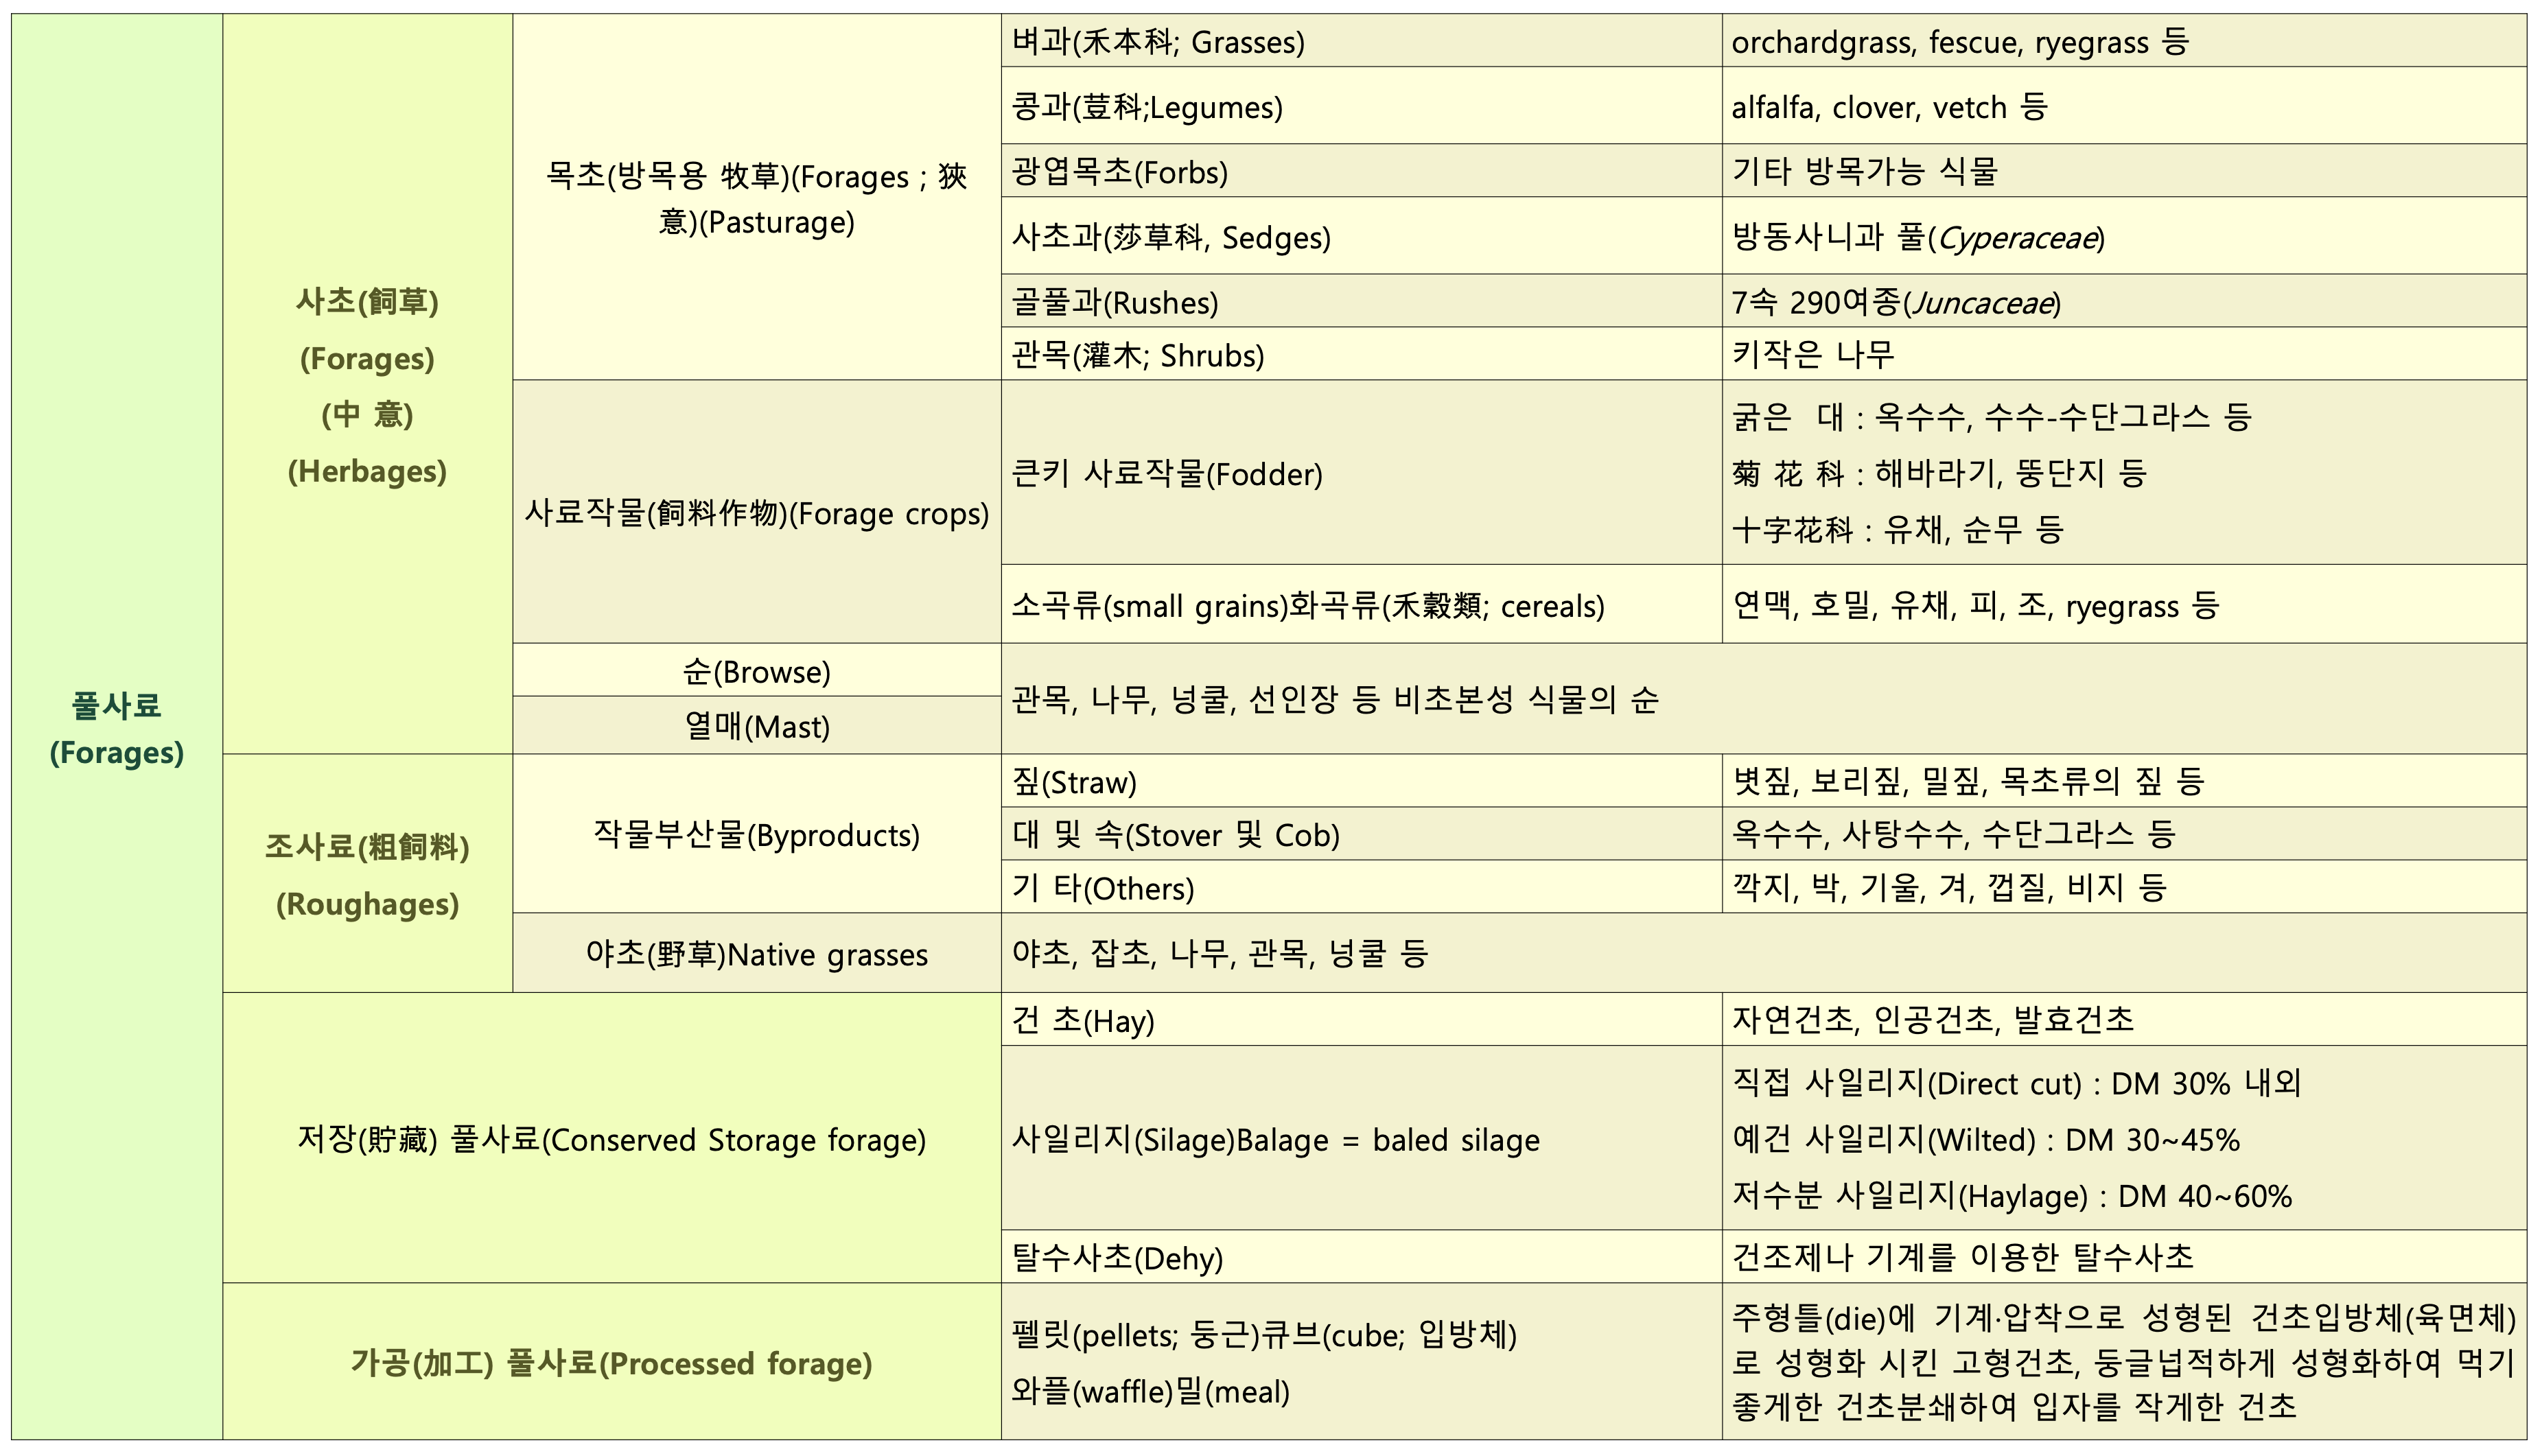
\includegraphics{figures/classification.png}

\section{풀사료의 평가}\label{-}

\subsection{풀사료를 평가하는 이유}\label{--}

\begin{itemize}
\tightlist
\item
  풀사료를 가장 효과적으로 이용하고 생산성을 최대로 높이기 위하여
\item
  영양가의 차이가 매우 심하기 때문(단백질 함량 : 알팔파; 10∼25\%, 벼과
  건초; 4∼20\%)
\item
  가축의 영양소 요구량은 천차만별(축종, 시기, 상태 등). 즉, 생산성이
  높거나 영양소 요구량이 많을때 가장 좋은 풀사료를, 요구량이 낮은
  가축이나 시기에는 저질의 풀사료 급여하는 것이 경제적이기 때문
\item
  시장의 올바른 유통을 위하여(객관적인 유통가격 결정자료로 이용되어,
  풀사료에 대한 정확한 지식이 없는 농가의 피해를 줄이기 위함)
\item
  올바른 사료배합(특정가축의 요구량에 맞는 사료를 배합할 때 어느 사료를
  얼마만큼 넣는 것이 경제적인지를 판단하는 자료로 이용)
\item
  단위면적당 생산성을 높이기 위하여
\end{itemize}

\subsection{평가방법}

\begin{enumerate}
\def\labelenumi{\arabic{enumi}.}
\tightlist
\item
  관능검사(官能檢査, visual appraisal, Physical : 사람의 오감(五感)을
  통하여 평가하는 방법),
\item
  화학적 분석(Chemical analysis)
\item
  근적외선 분광측정기(NIRS; Near infrared reflectance spectroscopy)
\item
  \emph{In vivo} 및 \emph{in vitro}
\item
  사양시험(digestion or feeding trial)
\end{enumerate}

\subsection{풀사료의 영양가치에 영향을 미치는 요인}\label{----}

\begin{itemize}
\tightlist
\item
  초종과 품종(Plant species and variety)
\item
  숙기(Maturity)
\item
  잎의 비율(Leafiness)
\item
  수확(Harvest)
\item
  저장(Storage) 방법과 저장 기술
\item
  환경(Environment)
\end{itemize}

\subsection{축우사료에서 풀사료의 중요성}\label{--}

\subsubsection{반추가축의 소화생리}\label{-}

\textbf{가. 반추위내의 미생물의 기능}

\begin{itemize}
\tightlist
\item
  섬유소의 분해\\
\item
  아미노산의 합성\\
\item
  Vit. B, K의 합성\\
\item
  미생물유체로서 영양소의 공급
\end{itemize}

\textbf{나. 반추위의 소화율}

\textbf{다. 반추위 내에서의 사료의 소화}

\begin{itemize}
\tightlist
\item
  휘발성지방산(VFA, volatile fatty acid))의 생성\\
\item
  조사료 위주 : 반추위의 초산 증가(초산 : 에너지원, 유지방합성 원료)\\
\item
  농후사료 위주 : 반추위의 프로피온산 증가(프로피온산 : 에너지원,
  체지방합성 원료)
\end{itemize}

\subsubsection{반추위의 정의와 발달}\label{--}

\begin{itemize}
\tightlist
\item
  반추위: 반추동물의 제1위와 제2위(1위만을 의미하기도 함). 1위와 2위는
  큰 구멍으로 연결되어 있고 내용물 이동이 자유로우며 소화기능상의 차이가
  없음.
\item
  갓 태어났을 때 : 4위보다 작고 기능도 거의 없음. 미생물도 서식하지 않음
\item
  조사료 섭취 개시 후 : 급격히 발달이 촉진
\item
  생후 3개월 이후 제1위만의 무게가 체중의 20\%, 소화기관 중에서 가장 큰
  기관으로 성장
\item
  생후 6개월 이후 : 모든 위의 80\% 이상 차지.\\
\item
  조사료에 의한 물리적 자극.

  \begin{itemize}
  \tightlist
  \item
    성장 초기에 조사료를 충분히 공급하여야 반추위가 충실하게 발달
  \item
    육성기 사육방법이 중요한 이유.
  \end{itemize}
\end{itemize}

\subsection{풀사료의 특성 및 중요성}\label{---}

\begin{enumerate}
\def\labelenumi{\arabic{enumi}.}
\item
  사료가치: TDN과 CP의 함량은 농후사료에 비해 상대적을 낮으나,
  무기물(Ca, P, Cu 등) vitamin 등이 높고, 각종 영양소가 완벽하게 조화를
  이루고 있어, 단일사료로 급여하여도 안전한 생산에 문제가 없다.
\item
  정상적인 생리기능유지: 조사료부족시 소화기장해(제4위전위증, 제엽염,
  과산증, 과비증후군) 유지율저하, 번식장해 발생
\item
  자급조사료의 경우 경제성과 사료수급의 안정성 향상
\item
  \textbf{인간의 식량과 경합이 없다}
\end{enumerate}

\chapter{Classification}\label{classification}

\section{식물학적 분류}\label{-}

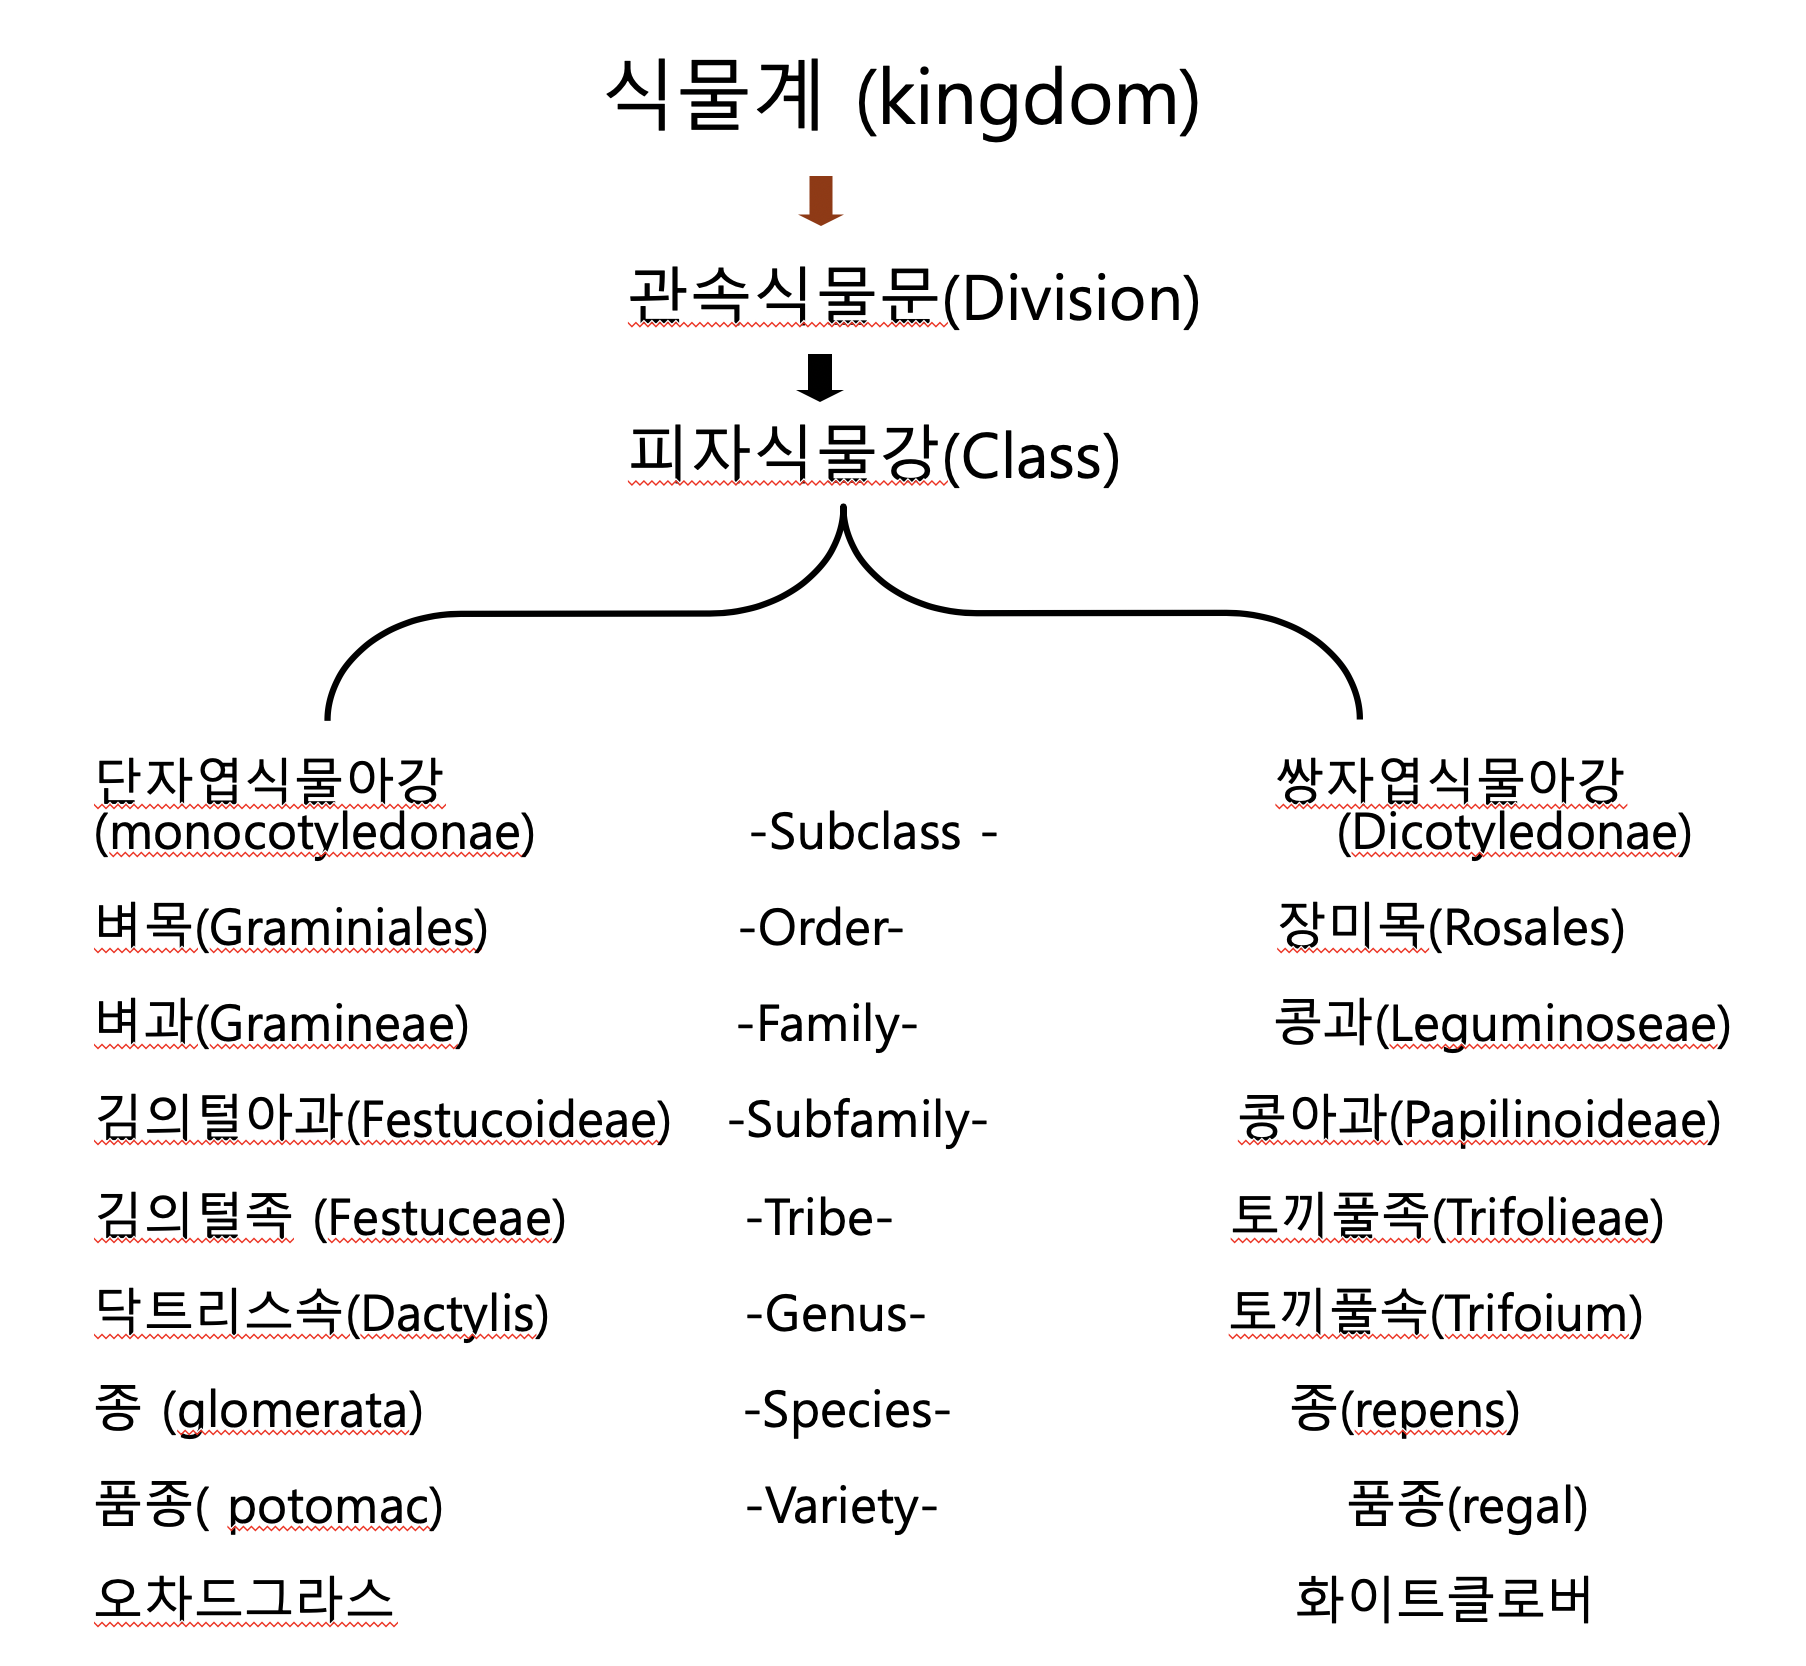
\includegraphics[width=400]{figures/kingdom}

\section{형태에 의한 분류}\label{--}

\begin{itemize}
\tightlist
\item
  벼(화본)과 사료작물: orchardgrass, timothy, tall fescue, 보리, 옥수수,
  밀, 벼, 수수, 피, 조
\item
  콩(두)과 사료작물: clover류, birdsfoot trefoil, vetch류, 콩, 완두
\item
  국과 사료작물: 해바라기, 돼지감자 등\\
\item
  십자화과 사료작물: 일반근채류(순무, 당근, 루타바카), 유채, 양배추
\item
  기타: 고구마 등
\end{itemize}

\subsection{벼과 사료작물}\label{-}

\subsubsection{벼과 사료작물의 특성}\label{--}

\begin{itemize}
\tightlist
\item
  사료작물의 약 75\% 점유
\item
  전세계적으로 600속, 약 5,000종 분포
\item
  \emph{Poaceae}과(벼과) 작물(\emph{Gramineae})
\item
  초본류 식물, 종자생산, 목질조직 발달미약
\item
  외떡잎 식물
\item
  다양한 초종의 분포
\item
  수량이 많고 방목이나 채초용으로 적합
\item
  재생력이 강하다
\item
  기호성이 좋고 영양가가 높다
\end{itemize}

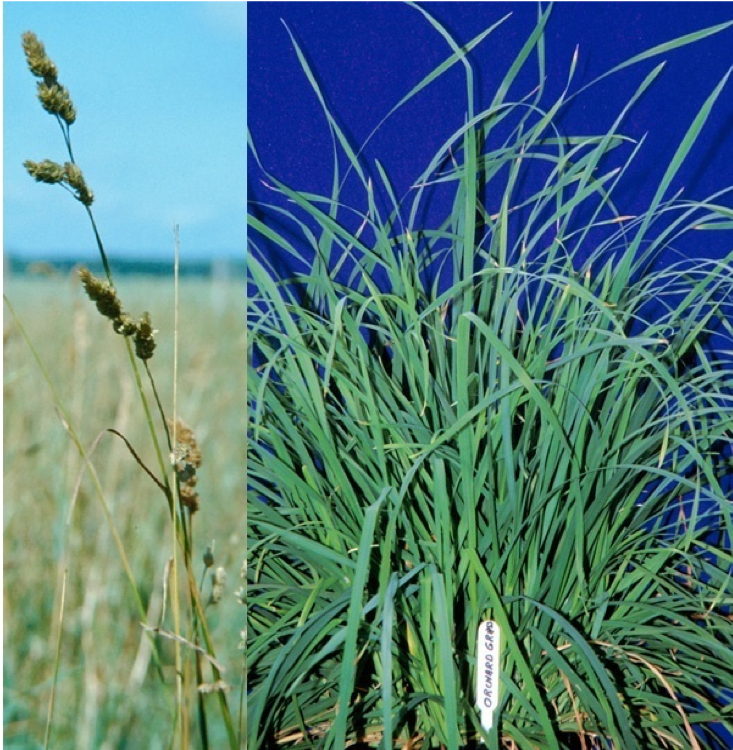
\includegraphics[width=400]{figures/grass1}

\subsubsection{벼과 목초의 일반적인 특징}\label{---}

\begin{itemize}
\tightlist
\item
  수염모양의 root system
\item
  줄기(stems)는 속이 비어있다
\item
  명확한 마디(node) 보유
\item
  잎(leaves)은 나란히맥이며, 마디마다 1잎씩 어긋난 형태
\item
  잎은 잎집(sheath), 잎몸(blade), 잎혀 (ligule), 잎귀(auricle)로 구성
\item
  꽃차례는 수상, 원추, 총상 꽃차례로 구성
\item
  꽃(flowers)은 3(1\textasciitilde{}3)개의 수술(雄蘂;stamen), 2개의
  인피(鱗被;lodicules), 1개의 암술(雌蘂;pistil)로 되어 있고 바깥쪽은
  내영(內穎; palea)과 외영(外穎;lemma)으로 되어 있다
\item
  일반적으로 외영은 1개의 까끄라기(awn)를 가지고 비스듬히 기울어져 있다
\item
  열매(fruit)는 씨방벽(子房壁;ovary wall)에 융합되어 있는 하나의 종자를
  가지고 있다
\item
  종자, 영양체(분얼,Tillering), 포복경(stolon), 지하경 (rhizome)에 의한
  번식
\end{itemize}

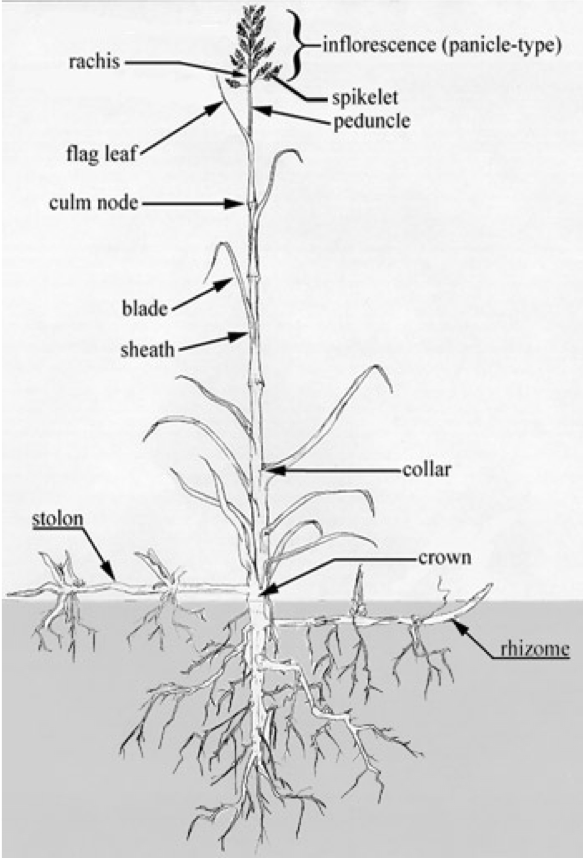
\includegraphics[width=300]{figures/grass2}

\section{기상연한에 의한 분류}\label{--}

\section{생존연한에 의한 분류}\label{--}

\section{이용형태에 의한 분류}\label{--}

\chapter{Grass and legume}\label{legumeandgrass}

\section{벼과 사료작물}\label{--1}

\subsection{가축사료로서의 중요성}\label{-}

\begin{itemize}
\tightlist
\item
  기호성이 우수하고 영양가가 높다
\item
  방목지나 채초지의 사초로써 그 가치가 높다
\item
  방목과 채초시 견디는 힘이 가장 강하다
\item
  전 세계적으로 가장 널리 분포하고 있다(600屬 5,000種).
\item
  가장 우세하게 자라며 중요 곡류의 대부분을 차지한다.
\item
  벼과를 ``Gramineae''라 부르며 ``벼과(Poaceae)''와
  ``대과(Bambusaceae)''로 나누기도 한다.
\item
  영어로는 ``grasses''라 하나 禾穀類(cereals)를 포함할 때는 ``forage
  grasses''라 한다.
\end{itemize}

\subsection{일반적 특성}\label{-}

\begin{itemize}
\tightlist
\item
  뿌리(根系; root system)는 수염뿌리로 되어 있다.
\item
  줄기(stem)은 대체로 속이 비어있고 둥글며, 두렷한 마디(節; node)가
  있다.
\item
  잎(葉, leaves)은 나란히 맥, 줄기위에 어긋나게 2열로 각 마디에 하나씩
  나 있다.
\item
  잎은 잎집(葉革+肖;sheath), 잎몸(葉身;blade), 잎혀(葉舌;ligule),
  잎귀(葉耳;auricle)로 구성되어 있다.
\item
  꽃차례(花序;inflorescence)는 수상(穗狀;spike), 원추(圓錐;panicle) 또는
  총상(總狀;raceme) 꽃차례로 되어 있다.
\item
  꽃(flowers)은 3(1\textasciitilde{}3)개의 수술(雄蘂;stamen), 2개의
  인피(鱗被;lodicules) 및 암술(雌蘂;pistil)로 되어 있으며 바깥족은
  내영(內穎;lemma)과 외영(外穎;palea) 2장으로 되어 있다.
\item
  열매(fruit)는 씨방벽(子房壁;ovary wall)에 융합되어 있는 하나의 종자를
  가지고 있다.
\end{itemize}

\subsection{형태적 특성}\label{-}

\begin{itemize}
\tightlist
\item
  방석형과 다발형 벼과 목초의 증식방법 : 종자, 영양체{[}분얼, 지하경,
  포복경, 비늘뿌리(鱗莖, haplocorm or corm){]}
\item
  방석형(sod former) 지하경(地下莖, 땅속기는줄기, Rhizomes)이나
  포복경(匍匐莖, 땅위기는줄기, Stolons)이 있는 초종
\end{itemize}

\chapter{Distinguishment}\label{distinguishment}

\chapter{Seed production}\label{seed-production}

\bibliography{book.bib,packages.bib}


\end{document}
